% THIS DOCUMENT IS FOLLOWS THE VOLERE TEMPLATE BY Suzanne Robertson and James Robertson
% ONLY THE SECTION HEADINGS ARE PROVIDED
%
% Initial draft from https://github.com/Dieblich/volere
%
% Risks are removed because they are covered by the Hazard Analysis
\documentclass[12pt]{article}

\usepackage{booktabs}
\usepackage{tabularx}
\usepackage{hyperref}
\usepackage{enumitem}
\usepackage{graphicx}
\usepackage{float} 

\hypersetup{
    bookmarks=true,         % show bookmarks bar?
      colorlinks=true,      % false: boxed links; true: colored links
    linkcolor=red,          % color of internal links (change box color with linkbordercolor)
    citecolor=green,        % color of links to bibliography
    filecolor=magenta,      % color of file links
    urlcolor=cyan           % color of external links
}

\newcommand{\lips}{\textit{Insert your content here.}}

%% Comments

\usepackage{color}

\newif\ifcomments\commentstrue %displays comments
%\newif\ifcomments\commentsfalse %so that comments do not display

\ifcomments
\newcommand{\authornote}[3]{\textcolor{#1}{[#3 ---#2]}}
\newcommand{\todo}[1]{\textcolor{red}{[TODO: #1]}}
\else
\newcommand{\authornote}[3]{}
\newcommand{\todo}[1]{}
\fi

\newcommand{\wss}[1]{\authornote{magenta}{SS}{#1}} 
\newcommand{\plt}[1]{\authornote{cyan}{TPLT}{#1}} %For explanation of the template
\newcommand{\an}[1]{\authornote{cyan}{Author}{#1}}

%% Common Parts

\newcommand{\progname}{ProgName} % PUT YOUR PROGRAM NAME HERE
\newcommand{\authname}{Team \#, Team Name
\\ Student 1 name
\\ Student 2 name
\\ Student 3 name
\\ Student 4 name} % AUTHOR NAMES                  

\usepackage{hyperref}
    \hypersetup{colorlinks=true, linkcolor=blue, citecolor=blue, filecolor=blue,
                urlcolor=blue, unicode=false}
    \urlstyle{same}
                                


\begin{document}

\title{Software Requirements Specification for \progname: subtitle describing software} 
\author{\authname}
\date{\today}
	
\maketitle

~\newpage

\pagenumbering{roman}

\tableofcontents

~\newpage

\section*{Revision History}

\begin{tabularx}{\textwidth}{p{3cm}p{2cm}X}
\toprule {\textbf{Date}} & {\textbf{Version}} & {\textbf{Notes}}\\
\midrule
Date 1 & 1.0 & Notes\\
Date 2 & 1.1 & Notes\\
\bottomrule
\end{tabularx}

~\\

~\newpage
\section{Purpose of the Project}
\subsection{User Business}
\lips
\subsection{Goals of the Project}
\lips
\section{Stakeholders}
\subsection{Client}
\lips
\subsection{Customer}
\lips
\subsection{Other Stakeholders}
\lips
\subsection{Hands-On Users of the Project}
\lips
\subsection{Personas}
\lips
\subsection{Priorities Assigned to Users}
\lips
\subsection{User Participation}
\lips
\subsection{Maintenance Users and Service Technicians}
\lips

\section{Mandated Constraints}
\subsection{Solution Constraints}
\begin{enumerate}[label=MD-SL \arabic*., wide=0pt, leftmargin=*]
  \item \emph{The solution design must comply with at least the Level AA of the Web Content Accessibility Guidelines (WCAG) 2.1 standards}\\[2mm]
    {\bf Rationale:} This ensures that the solution ensures inclusivity for users with visual, auditory, or cognitive impairments\\
    {\bf Fit Criterion:} The solution must past all tests using WCAG automated testing tools and manual tests.\\
    {\bf Priority:} High
\end{enumerate}
\begin{enumerate}[label=MD-SL \arabic*., wide=0pt, leftmargin=*]
  \item \emph{The solution must be implemented as a website}\\[2mm]
    {\bf Rationale:} A website will allow for automated testing against the WCAG standards which ensures accesibility for users 
    and allow users to upload images/figures to generate alternative text\\
    {\bf Fit Criterion:} The website must be functional and allow users to generate alternative text by uploading
    images and figures\\
    {\bf Priority:} High
\end{enumerate}
\begin{enumerate}[label=MD-SL \arabic*., wide=0pt, leftmargin=*]
  \item \emph{The solution must support common image formats (e.g. JPEG, PNG, etc.)}\\[2mm]
    {\bf Rationale:} The website will enable users to upload images or figures to generate the alternative text, therefore the solution must be able 
    to handle the different types of image formats\\
    {\bf Fit Criterion:} The product must successfully process at least one image of each required format including JPEG and PNG
    images and figures\\
    {\bf Priority:} High
\end{enumerate}

\subsection{Implementation Environment of the Current System}
\begin{enumerate}[label=MD-IE \arabic*., wide=0pt, leftmargin=*]
  \item \emph{The product must be able to run on standard laptop environments, including operatins systems (OS) such as 
  macOS, Windows, and Linux}\\[2mm]
    {\bf Rationale:} This ensures that the product is compatible with major operating systems to allow the product to be 
    accessible to users, regardless of their laptop environment\\
    {\bf Fit Criterion:} The product must successfully install and operate on the latest releases of macOS, Windows, and Linux,
    verified through installation and functionality testing on each OS\\
    {\bf Priority:} High
\end{enumerate}
\subsection{Partner or Collaborative Applications}
\begin{enumerate}[label=MD-PA \arabic*., wide=0pt, leftmargin=*]
  \item \emph{The product must not conflict with other accessibility tools (e.g. screen readers, screen magnifiers, dictation software)}\\[2mm]
    {\bf Rationale:} This is to ensure that the product does not limit or intefere with other accessibility tools that 
    meets the users' needs \\
    {\bf Fit Criterion:} The product must operate simultaneously with at least one other accessibility tool,
    verified through interoperability testing \\
    {\bf Priority:} High
\end{enumerate}
\subsection{Off-the-Shelf Software}
\lips
\subsection{Anticipated Workplace Environment}
The anticipated workplace environment for this product is academic settings such as universities, where students may 
require alternative text to interpret images and figures within their coursework and study materials.
\subsection{Schedule Constraints}
\begin{enumerate}[label=MD-SC \arabic*., wide=0pt, leftmargin=*]
  \item \emph{The final product must be completed and tested by the end of the academic term (April 2025)}\\[2mm]
    {\bf Rationale:} This is to ensure that the final product is functional and meets all requirements
    at the end of the academic year\\
    {\bf Fit Criterion:} All deliverables are submitted, and the final product is tested and operable by April 2025 \\
    {\bf Priority:} High
\end{enumerate}
\subsection{Budget Constraints}
\begin{enumerate}[label=MD-BC \arabic*., wide=0pt, leftmargin=*]
  \item \emph{The project budget must include compensation for user testers, set at maximum \$150 per participant for two rounds of usability testing.}\\[2mm]
    {\bf Rationale:} This is to ensure that user testers are compensated for their meaningful feedback, 
    and that our testing aligns with ethical practices\\
    {\bf Fit Criterion:} There must be record of participants being compensated between the range of \$100 and \$150 for
    two rounds of testing. \\
    {\bf Priority:} High
\end{enumerate}
\subsection{Enterprise Constraints}
\begin{enumerate}[label=MD-EC \arabic*., wide=0pt, leftmargin=*]
  \item \emph{The product must comply with the Accessibility for Ontarians with Disabilities Act (AODA)}\\[2mm]
    {\bf Rationale:} This ensures that the product meets the legal requirements in Ontario and guarantees that 
    the product is accessible to users with diverse needs\\
    {\bf Fit Criterion:} AODA requires compliance with WCAG standards, which ensures that the product meets AODA regulations. 
    Compliance must be verified through both automated WCAG testing tools and manual accessibility testing.\\
    {\bf Priority:} High
\end{enumerate}

\section{Naming Conventions and Terminology}
\subsection{Glossary of All Terms, Including Acronyms, Used by Stakeholders
involved in the Project}
\lips

\section{Relevant Facts And Assumptions}
\subsection{Relevant Facts}
\begin{itemize}
  \item This project is being developed for a Software Engineering Capstone course with a fixed timeline
  \item The solution is targeted primarily for laptop and/or desktop environments, but can later be extended for mobile platforms use
\end{itemize}
\subsection{Business Rules}
The business rules established among the team are as follows: 
\begin{itemize}
  \item \textbf{Adherence to Project Schedule}: All deliverables and milestones must be 
  completed according to the established project schedule. Any anticipated delays must be communicated
  in advance.
  \item \textbf{Pull Request Requirement}: All pull requests made by a team member must be reviewed by 
  three other members before being merged into the \texttt{main} branch. The reviewers must provide approval
  or feedback within 24 hours of the pull request.
  \item \textbf{Team Communication Standard}: All team members must communicate respectfully and professionally during 
  all discussions, meetings, and written communication. 
  \item \textbf{Testing Requirements}: All code contributions must include appropriate unit, intergration, and 
  functionality tests to ensure correctness and reliability. Accessibility testing must also be performed for all
  product features. 
\end{itemize}
\subsection{Assumptions}
The following assumptions are made when using the product:
\begin{itemize}
  \item Users will be operating on modern browsers such as Chrome, Safari, and Firefox
  \item Users will have access to stable internet connection when installing and using the product
  \item Users will have basic knowledge of installing and enabling web extensions
\end{itemize}
\section{The Scope of the Work}
\subsection{The Current Situation}
Currently, alternative text generation tools are able to provide sufficient descriptions for simple images and figures. However, for more complex visuals 
such as engineering diagrams, the generated alt text is often misleading, incomplete, or inefficient at conveying the intended meaning.\\
Accurate alternative text is particularly essential for individuals with visual or cognitive impairments, as it enables fair access to academic content. Without 
reliable descriptions, students may experience barriers to learning and miss critical information conveyed in diagrams and figures.\\
The current limitations of existing generated alternative text tools are as follows:
\begin{itemize}
  \item \textbf{Inaccurate Alternative Text}: Generated alt text may emphasize unimportant details and overlook key elements, 
  resulting in misleading or confusing interpretations.
  \item \textbf{Oversimplification of Complex Figures}: Current tools frequently oversimplify technical or academic diagrams, 
  failing to capture essential details required for learning.
  \item \textbf{High Manual Effort}: In many cases, subject matter experts must manually create alt text, 
  which is time-intensive and not scalable across large volumes of academic content.
\end{itemize}
\subsection{The Context of the Work}
The product will be in the form of a website that integrates into existing accessibility workflows
by providing accurate descriptions from images that can be read aloud by screen readers. The product 
will complement existing screen readers by ensuring accurate generated alternative text from 
uploaded images and figures of academic work are available. \href{fig:work-context}{Figure1} shows 
how the product will integrate with existing screen readers.\\
\begin{figure}[h]
  \centering
  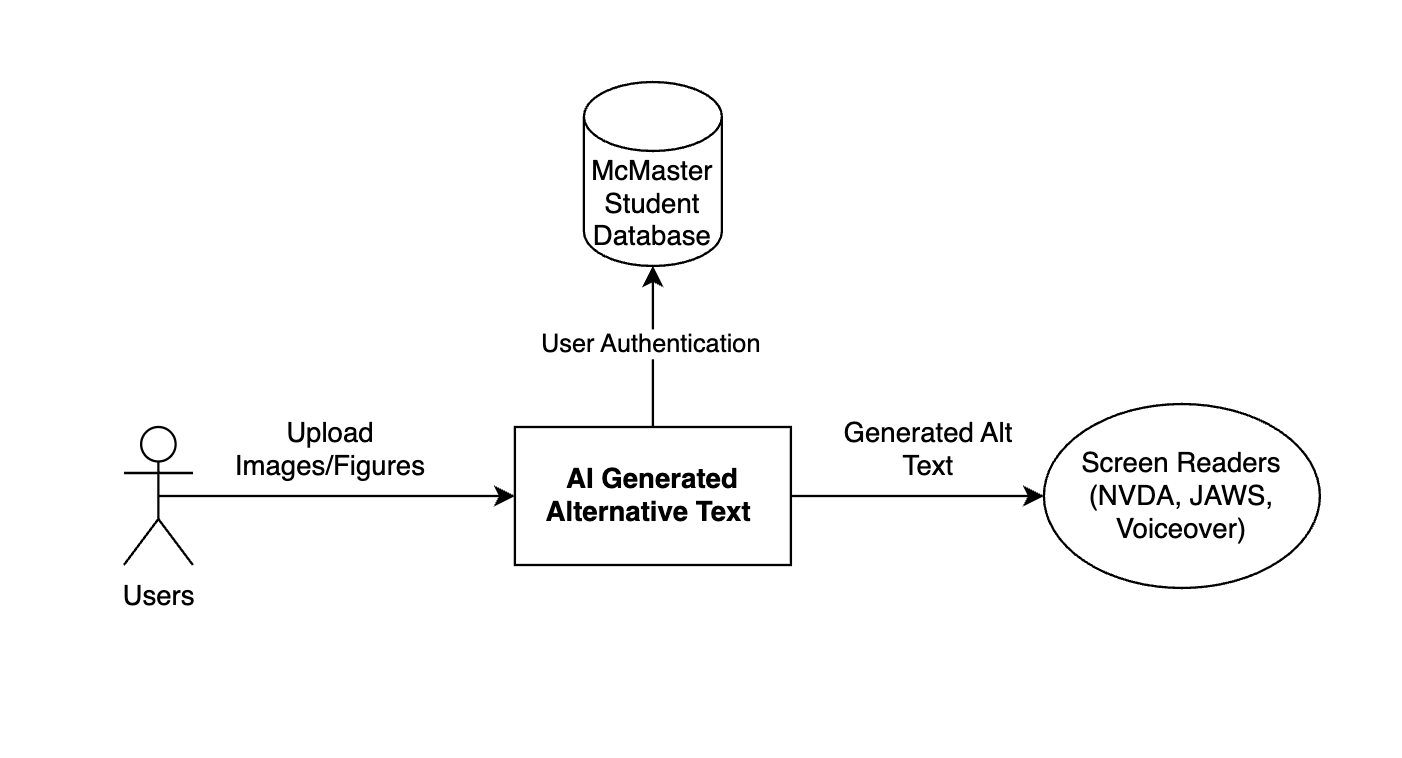
\includegraphics[width=1.0\textwidth]{images/work-context-diagram.png}
  \caption{Work Context Diagram}
  \label{fig:work-context}
\end{figure}

\subsection{Work Partitioning}
\href{tab:work-partition}{Table 1} shows the work partitioning for completing the project. It includes major events, 
their inputs and outputs, and the summary of the event.

\begin{table}[H]
  \centering
  \caption{Work Partition for the System}
  \label{tab:work-partition}
  \begin{tabular}{ |p{3cm}|p{3cm}|p{3cm}|p{4cm}| }
    \hline
    \textbf{Event Name} & \textbf{Input} & \textbf{Output} & \textbf{Summary} \\
    \hline
    Login & Username, Password & & User logs in using their McMaster account \\
    \hline
    Upload  \mbox{Images/Figures} & PNG/JPEG files & Uploaded File Reference & User uploads their files to generate alternative text \\
    \hline
    \mbox{OCR Text} \mbox{Extraction} & Uploaded \mbox{Images/Figures} & Detected Text & System reads the text embedded in the uploaded files \\
    \hline
    Generate \mbox{Alternative Text} & Uploaded  \mbox{Images/Figures}, Extracted OCR, Model Parameters & Generated Alt Text, Quality Metric from ML Model & System analyzes the image and extracted OCR data to generate accurate alternative text \\
    \hline
    View History & \mbox{User Login,} Stored Uploads and Generated Alt Text & List of Previously Generated Alt Text & The system retrieves and displays a user’s history of uploaded images along with their associated generated alt text \\
    \hline
  \end{tabular}
\end{table}


\subsection{Specifying a Business Use Case (BUC)}
\lips

\section{Business Data Model and Data Dictionary}
\subsection{Business Data Model}
\lips
\subsection{Data Dictionary}
\lips

\section{The Scope of the Product}
\subsection{Product Boundary}
\lips
\subsection{Product Use Case Table}
\lips
\subsection{Individual Product Use Cases (PUC's)}
\lips

\section{Functional Requirements}
\subsection{Functional Requirements}
\lips

\section{Look and Feel Requirements}
\subsection{Appearance Requirements}
\lips
\subsection{Style Requirements}
\lips

\section{Usability and Humanity Requirements}
\subsection{Ease of Use Requirements}
\lips
\subsection{Personalization and Internationalization Requirements}
\lips
\subsection{Learning Requirements}
\lips
\subsection{Understandability and Politeness Requirements}
\lips
\subsection{Accessibility Requirements}
\lips

\section{Performance Requirements}
\subsection{Speed and Latency Requirements}
\lips
\subsection{Safety-Critical Requirements}
\lips
\subsection{Precision or Accuracy Requirements}
\lips
\subsection{Robustness or Fault-Tolerance Requirements}
\lips
\subsection{Capacity Requirements}
\lips
\subsection{Scalability or Extensibility Requirements}
\lips
\subsection{Longevity Requirements}
\lips

\section{Operational and Environmental Requirements}
\subsection{Expected Physical Environment}
\lips
\subsection{Wider Environment Requirements}
\lips
\subsection{Requirements for Interfacing with Adjacent Systems}
\lips
\subsection{Productization Requirements}
\lips
\subsection{Release Requirements}
\lips

\section{Maintainability and Support Requirements}
\subsection{Maintenance Requirements}
\lips
\subsection{Supportability Requirements}
\lips
\subsection{Adaptability Requirements}
\lips

\section{Security Requirements}
\subsection{Access Requirements}
\lips
\subsection{Integrity Requirements}
\lips
\subsection{Privacy Requirements}
\lips
\subsection{Audit Requirements}
\lips
\subsection{Immunity Requirements}
\lips

\section{Cultural Requirements}
\subsection{Cultural Requirements}
\lips

\section{Compliance Requirements}
\subsection{Legal Requirements}
\lips
\subsection{Standards Compliance Requirements}
\lips

\section{Open Issues}
\lips

\section{Off-the-Shelf Solutions}
\subsection{Ready-Made Products}
\lips
\subsection{Reusable Components}
\lips
\subsection{Products That Can Be Copied}
\lips

\section{New Problems}
\subsection{Effects on the Current Environment}
\lips
\subsection{Effects on the Installed Systems}
\lips
\subsection{Potential User Problems}
\lips
\subsection{Limitations in the Anticipated Implementation Environment That May
Inhibit the New Product}
\lips
\subsection{Follow-Up Problems}
\lips

\section{Tasks}
\subsection{Project Planning}
\lips
\subsection{Planning of the Development Phases}
\lips

\section{Migration to the New Product}
\subsection{Requirements for Migration to the New Product}
\lips
\subsection{Data That Has to be Modified or Translated for the New System}
\lips

\section{Costs}
\lips
\section{User Documentation and Training}
\subsection{User Documentation Requirements}
\lips
\subsection{Training Requirements}
\lips

\section{Waiting Room}
\lips

\section{Ideas for Solution}
\lips

\newpage{}
\section*{Appendix --- Reflection}

The purpose of reflection questions is to give you a chance to assess your own
learning and that of your group as a whole, and to find ways to improve in the
future. Reflection is an important part of the learning process.  Reflection is
also an essential component of a successful software development process.  

Reflections are most interesting and useful when they're honest, even if the
stories they tell are imperfect. You will be marked based on your depth of
thought and analysis, and not based on the content of the reflections
themselves. Thus, for full marks we encourage you to answer openly and honestly
and to avoid simply writing ``what you think the evaluator wants to hear.''

Please answer the following questions.  Some questions can be answered on the
team level, but where appropriate, each team member should write their own
response:

\textbf{Group Reflection  - Reflection}
\begin{enumerate}
  \item What went well while writing this deliverable? 
  
  Throughout the process, our team maintained organization and had good communication.  It was simpler to preserve flow and prevent redundancy because we had a clear framework and consistent formatting from earlier deliverables.  We were also able to maintain our efficiency and keep the material consistent with our previous work.  In order review sections, define expectations, and make sure the deliverable satisfied all requirements, we also had meetings with our TA and our team.
  \item What pain points did you experience during this deliverable, and how did
  you resolve them?

  One difficulty was avoiding redundancy by keeping formatting constant and clearly distinguishing design components from implementation specifics. In order to guarantee accuracy and uniformity throughout all sections, we addressed this by going over the course templates and conducting team editing sessions to make sure the formatting followed a consistent style. We also helped each other out by sharing tips and tricks to improve clarity and presentation.

  \item How many of your requirements were inspired by speaking to your
  client(s) or their proxies (e.g. your peers, stakeholders, potential users)?
  
  Key design and functionality components that were influenced by internal meetings, conversations with our supervisor, pertinent compliance guidelines, and my internship's prior experience working with AI included the accessible interface, the quality of the alt text that was generated, and adherence to AODA and WCAG 2.1 standards.
  \item Which of the courses you have taken, or are currently taking, will help
  your team to be successful with your capstone project.

  The Software Requirements course from third year was extremely useful in creating this deliverable.  It created a solid foundation for organizing requirement documents, developing precise specifications, and grasping the foundations of software documentation and traceability, all of which significantly aided our work on this project.

  \item What knowledge and skills will the team collectively need to acquire to
  successfully complete this capstone project?  Examples of possible knowledge
  to acquire include domain specific knowledge from the domain of your
  application, or software engineering knowledge, mechatronics knowledge or
  computer science knowledge.  Skills may be related to technology, or writing,
  or presentation, or team management, etc.  You should look to identify at
  least one item for each team member.}\newline
  
  \item \textbf{For each of the knowledge areas and skills identified in the previous
  question, what are at least two approaches to acquiring the knowledge or
  mastering the skill?  Of the identified approaches, which will each team
  member pursue, and why did they make this choice?}\newline

\end{enumerate}


\textbf{Moly Mikhail  - Reflection}
\begin{enumerate}
  \item \textbf{What went well while writing this deliverable?} \newline
  I believe writing this deliverable many things went well. I really enjoyed getting to think about the different
  non-functional requirements. I found that have different sections of non-functional requirements encouraged me to think about different 
  aspects of the system and things we will have to keep in mind during development. For example, prior to writing 
  this deliverable, we hadn’t considered personalization and internationalization requirements; however, having to
  complete that section led us to add important functionality of allowing the user to decide which way
  to store the alternative text. 
  
\item \textbf{What pain points did you experience during this
    deliverable, and how did you resolve them?} \newline
  One pain point I experience writing this deliverable dealt with completing the product boundary. 
  Initially, I was confused on The Scope of the Product section and what was expected. 
  To resolve this, I researched the Volere Requirements Specification Template and looked into the section. 
  However, I was still confused and what was expected of the section. Finally, during our meeting with
  our TA I was able to clarify the expectations for this section and I was able to complete the section. 
 
   \item \textbf{How many of your requirements were inspired by
      speaking to your client(s) or their proxies (e.g., your peers,
    stakeholders, potential users)?} \newline
  I believe many of our non-functional requirements, specifically look and feel 
  requirements, as well as usability and humanity requirements. Through our
  conversations with our supervisor Jing, we learned a lot of the accessibility
  requirements for website applications. For example, one specific requirement 
  that was derived from our conversations was that the system cannot use color alone to convey any messages
  or information. I believe without having this conversation, this is a requirement that would not have been discovered. 
 
 \item \textbf{Which of the courses you have taken, or are currently
      taking, will help your team be successful with your capstone
    project?} \newline
  I believe many courses that I have taken, and some that I’m currently taking will 
  contribute to the success of our capstone project. I completed
  SFWRENG 4HC3 - Human Computer Interfaces, which has taught me many 
  important design principles, such as Normans Design Principles. Furthermore, 
  completing COMPSCI 4AL3 - Applications of Machine Learning, also will be a lot of help when 
  completing our capstone. This course introduced me to developing machine learning models and 
  will be directly applicable. Finally, taking COMPSCI 3RA3 - Software Requirements and Security 
  Considerations will also help our team be successful. 
  
\end{enumerate}

\textbf{Casey Francine Bulaclac - Reflection}
\begin{enumerate}
  \item \textbf{What went well while writing this deliverable?} \newline
  Having discussed the project thoroughly as a team and with our supervisor helped in writing this deliverable as the team
  was very knowledgeable about the needs for the project. 
  This deliverable went much smoother than the last due to stronger operational procedures, and better organization in how we structured and completed the SRS. 
  The team communicated well and were clear of the goals for this deliverable.
  \item \textbf{What pain points did you experience during this
  deliverable, and how did you resolve them?} \newline
  One pain point in writing the SRS was figuring out what each of the many sections entailed in the Volere's template. The template 
  is very thorough and needed many details, in which some sections seem to overlap which can be confusing. Another pain point was ensuring traceability
  between our goals in the project and the requirements. To resolve this, I made sure to ask the TA for feedback and clarification about specific sections.
  Additionally, communicating with each team member and ensuring our requirements aligned to the goals of the project was very helpful in aiding to ensure
  traceability.
\item \textbf{How many of your requirements were inspired by
      speaking to your client(s) or their proxies (e.g., your peers,
    stakeholders, potential users)?} \newline
  Many, if not most, requirements were inspired through speaking with our supervisor, who had the most knowledge and experience with our project's 
  potential users and stakeholders. In this project, it is important to understand our target users as we are designing for accessibility, so it was critical 
  in making our requirements. 
 \item \textbf{Which of the courses you have taken, or are currently
      taking, will help your team be successful with your capstone
    project?} \newline
  In this deliverable, the course that was most beneficial was Software Requirements and Security Considerations (SFWRENG 3RA3) as we learned how to create effected SRS documents.
  A course I've taken that will help thoroughly in ensuring our user interface is accessible is Human Computer Interfaces (SFWRENG 4HC3) as the course taught us principles of good design. Lastly,
  another course I took that contribute to the success of our project is Applications of Machine Learning (SFWRENG 4AL3) as this project heavily involves machine learning
  in generating alternative text. 
\end{enumerate}

\end{document}